\documentclass[preprint2, twocolappendix]{aastex631}
\received{\today}
\shorttitle{Improved NEO Classification}
\graphicspath{{figures/}}

\usepackage{lipsum}
\usepackage{physics}
\usepackage{multirow}
\usepackage{xspace}
\usepackage{natbib}
\usepackage{fontawesome5}
\usepackage{xcolor}
\usepackage{wrapfig}
\usepackage[figuresright]{rotating}

% remove indents in footnotes
\usepackage[hang,flushmargin]{footmisc} 

\newcommand{\todo}[1]{{\color{red}{[TODO: #1}]}}
\newcommand{\needcite}{{\color{magenta}{(needs citation)}}}
\newcommand{\placeholder}[1]{{\color{gray} \lipsum[#1]}}

% custom function for adding units
\makeatletter
\newcommand{\unit}[1]{%
    \,\mathrm{#1}\checknextarg}
\newcommand{\checknextarg}{\@ifnextchar\bgroup{\gobblenextarg}{}}
\newcommand{\gobblenextarg}[1]{\,\mathrm{#1}\@ifnextchar\bgroup{\gobblenextarg}{}}
\makeatother

\newcommand{\dig}{\texttt{digest2}}
\newcommand{\sss}{S3M}
\newcommand{\mpco}{MPCORB}

\begin{document}

\title{{\large An improved classification scheme for distinguishing NEOs from MBAs}\\\vspace{0.15cm}ASTR 597A Final Project}

% affiliations
\newcommand{\UW}{Department of Astronomy, University of Washington, Seattle, WA, 98195}

\author[0000-0001-6147-5761]{Tom Wagg}
\affiliation{\UW}

\correspondingauthor{Tom Wagg}
\email{tomwagg@uw.edu}

% \begin{abstract}
%     todo
% \end{abstract}

\keywords{}

\section{Introduction}

\begin{figure}[htb]
    \centering
    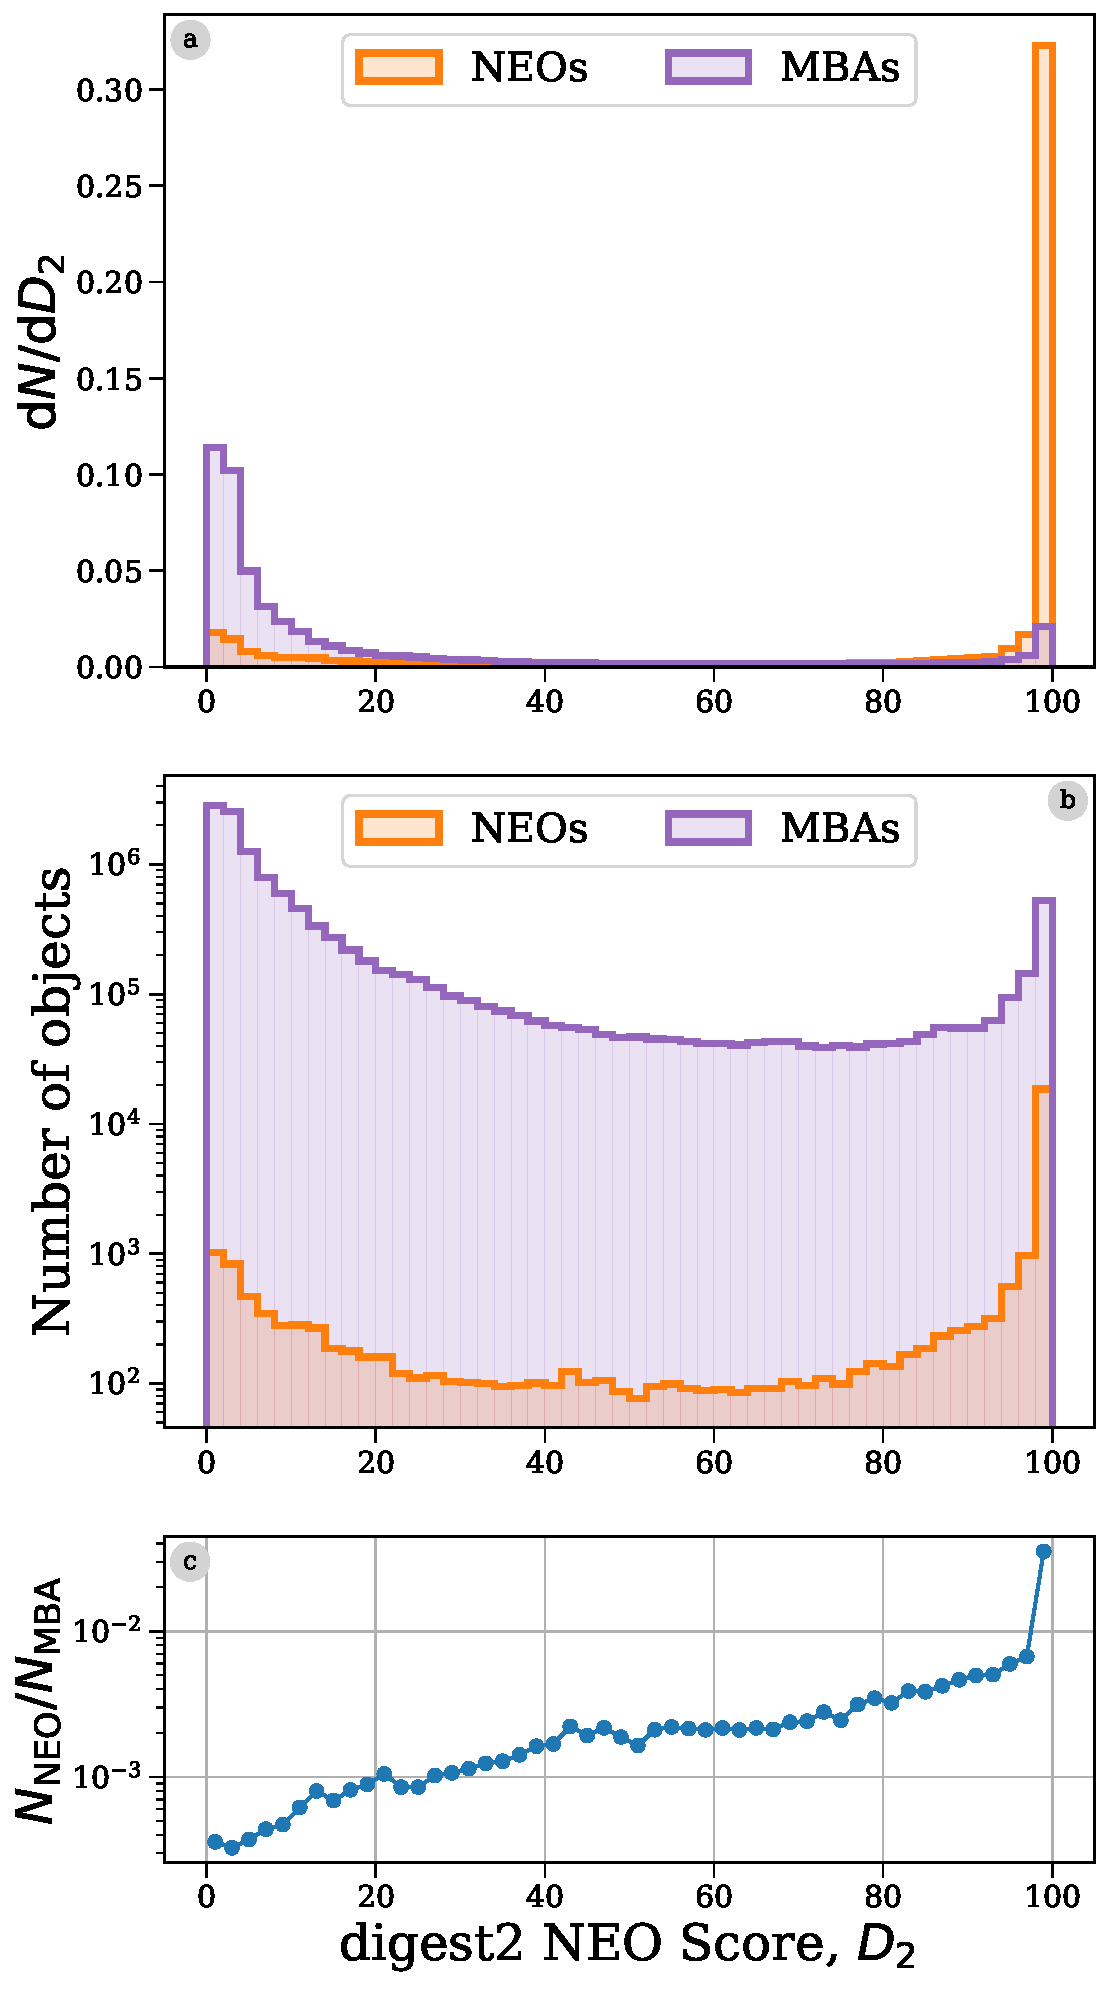
\includegraphics[width=\columnwidth]{digest2_pollution.pdf}
    \caption{\dig{} scores for all NEOs and MBAs observed in the first year of our simulated LSST observations. \textbf{(a)} normalised histograms of \dig{} scores, \textbf{(b)} the same histograms un-normalised \textbf{(c)} ratio of the histograms in (b). Note that the latter two panels are on a logarithmic scale.}
    \label{fig:digest2_should_be_scared}
\end{figure}

Near-Earth Objects (NEOs) are asteroids and comets that have a perihelion distance less than $1.3 \unit{au}$. It is estimated that approximately one fifth of this population passes close enough to Earth that small perturbations in their orbit may lead to intersections with the Earth's orbit and potential collisions \citep[e.g.][]{Jones+2018}. A subset of these objects are known as Potentially Hazardous Asteroids (PHAs), these objects are defined as being at least 140m in diameter that pass within 0.05au of the Earth\footnote{\url{https://cneos.jpl.nasa.gov/about/neo_groups.html}}. PHAs are large enough to make it through the Earth's atmosphere and still cause continent scale damage through impact. Given the threat posed by these objects, a world-wide effort\footnote{E.g.\,\url{https://www.unoosa.org/oosa/en/ourwork/topics/neos/index.html}} has been ongoing to catalogue and determine the orbits and sizes of NEOs including identifying any posing a hazard to the Earth.

The Minor Planet Center maintains a catalogue of known NEOs and their orbits\footnote{\url{https://www.minorplanetcenter.net/iau/MPCORB/NEA.txt}}, as well as the NEO confirmation page (NEOCP\footnote{\url{https://www.minorplanetcenter.net/iau/NEO/toconfirm_tabular.html}}). The NEOCP is a continously updated web page listing newly discovered NEO candidates that should be prioritised for additional observations by the NEO follow-up community. These follow-up observations contribute additional astrometric observations necessary to more accurately determine the orbit of the candidate, as well as photometry to constrain its size. An object is only listed on the NEOCP when it has a high probability of being an NEO. This probability is quantified using the \dig{} code \citep{Keys+2019}. \dig{} assigns a score between 0 and 100 based on potential orbits that fit the observations and only objects with a score of 65 or more are listed on the page. Currently, on average around two dozen objects are added to the NEOCP on each night.

The Rubin Observatory Legacy Survey of Space and Time \citep[LSST,][]{Ivezic+2019} will rapidly increase the rate at which NEO candidates are identified and reported to the NEOCP. \citet{Jones+2018} showed that at the end of the 10-year LSST baseline survey the completeness of NEOs with an absolute magnitude of $H \le 22$ would be 73\%. Most of these objects will be discovered using ``tracklet linking'': a computational technique where at least three pairs of observations (``tracklets'') observed over a 15-night period are identified as belonging to the same object (\citealp{Juric+2017}; Heinze et al., in prep). The orbits of objects discovered with this technique will typically be reasonably well known, and in need of no immediate follow-up. However, this tracklet linking comes at a cost: the object is not identified as interesting until the third tracklet is imaged -- at best, two nights after the first observation or, at worst, nearly two weeks later. This means that potentially interesting (or hazardous) objects may be missed until it's too late to observe (or react to) them.

The number of objects submitted to the NEOCP will increase by several orders of magnitude, and a large fraction of these submissions will be main belt asteriods (MBAs) \citep{sky-is-falling}. This would present difficulties for community follow-up, with too many available candidates (and of low purity) passing the current submission criteria.

Due to the vast MBA background, \dig{} performs poorly in identifying NEO candidates, as is demonstrated in Figure~\ref{fig:digest2_should_be_scared}. We show due to the extreme number of MBA submissions, only 1.5\% of submissions meeting the current criteria (a score of least 65) are NEOs, and only 10\% of objects with a perfect score of 100 are actually NEOs. Additionally, a large fraction of objects obtain a score of exactly 100 and it can be difficult to discriminate the best candidates among this group. It is clear that this classification scheme requires improvement.
\\

The aim of this paper is to augment \dig{} in classifying NEOs in the presence of a significant MBA background. We simulate one year of LSST observations on a synthetic solar system catalogue and calculate \dig{} scores for each tracklet. We investigate three additional parameters - ecliptic latitude, direction of motion relative to the ecliptic and apparent magnitude - as potential further discriminators between NEOs and MBAs in addition to the \dig{} score. We consider various combinations of these parameters to further refine submissions to the NEOCP and highlight how sorting submissions by these parameters can better identify high probability NEO candidates.

\section{Methods}

\subsection{Simulated tracklet population}

We create a population of simulated tracklets by performing mock LSST observations on the Synthetic Solar System Model \citep{Grav+2011}. We use a modified ``Baseline v2.1''\footnote{\url{https://community.lsst.org/t/survey-simulations-v2-1-april-2022/6538}} 10 year scheduler simulation strategy \citep{Naghib+2019, Cornwall+2020}. These observations account for both scheduled and unscheduled downtime and simulate the current baseline observing strategy that will be followed by LSST. The resulting simulations span 3653 days, and have over 50 million observations. The modification consists of shifting the start of LSST to March 2022, around the epoch of the MPCORB catalog used to generate the input hybrid catalogue dataset.

We select observations from the simulated LSST dataset that correspond to tracklets. For a tracklet to be built, we require it to satisfy the following criteria:
\begin{enumerate}
    \item \textbf{Number of observations:} We consider only objects which have at least 3 observations on a given night.
    \item \textbf{Maximum time separation:} We set the maximum time between observations to 90 minutes.
    \item \textbf{Minimum arc length:} We ensure that each tracklet is at least 1 arcsecond in length.
\end{enumerate}
The motivation behind these cuts is to ensure that the tracklet constrains the on-sky motion of the object sufficiently well, so that its position at a later time can be easily extrapolated. With fewer observations or shorter tracklets, many different orbits could reproduce the same motion on the sky. Moreover, observations that are separated too significantly in time may be spurious linkages, where observations of multiple objects are incorrectly assumed to be of the same source.

\subsection{Additional NEO scoring parameters}

\begin{figure}[htb]
    \centering
    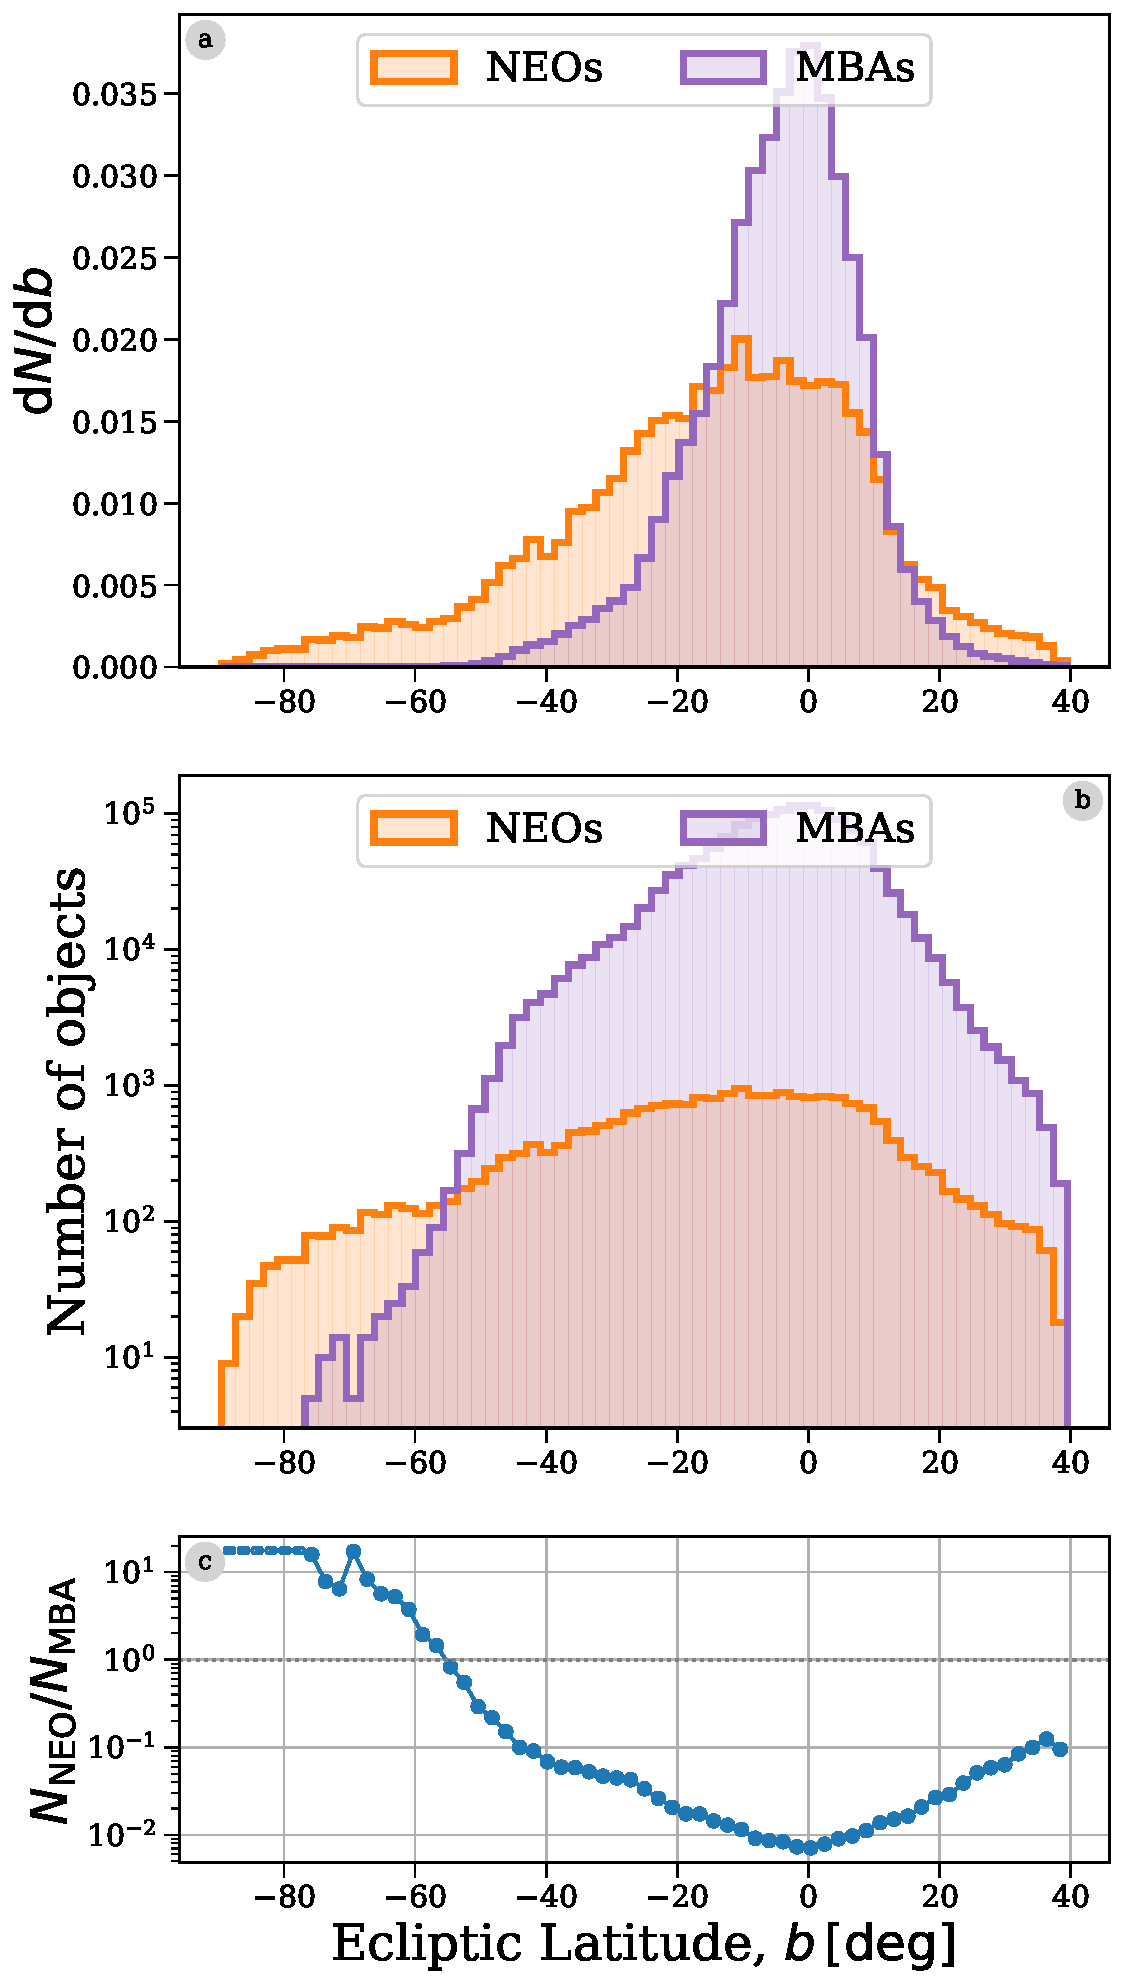
\includegraphics[width=\columnwidth]{figures/ecliptic_latitude_dist_highscore.pdf}
    \caption{As Figure~\ref{fig:digest2_should_be_scared}, but for ecliptic latitude and only for observations with a \dig{} score of at least 65.}
    \label{fig:ecl_lat_highscore}
\end{figure}

In addition to the orbital parameters used in computing the \dig{} score, we propose 3 additional parameters to consider in scoring NEOs: ecliptic latitude, direction of motion relative to the ecliptic plane and apparent magnitude. These parameters are motivated by the fact that MBAs are constrained to lie within the ecliptic plane around 3au from the Sun, whereas NEOs are often much closer and are not constrained to any location in the ecliptic.

For these reasons, one would predict that an object with a large ecliptic latitude is less likely to be a MBA. We explore this in Figure~\ref{fig:ecl_lat_highscore}, in which we show the distribution of ecliptic latitudes for objects with a \dig{} score of at least 65. As expected, we find that MBAs are concentrated around the ecliptic plane, whereas NEOs extend to the survey limits in either direction. In particular, we note that even without normalising the histogram, NEOs dominate over MBAs below an ecliptic latitude of $-55^{\circ}$.

\begin{figure}[htb]
    \centering
    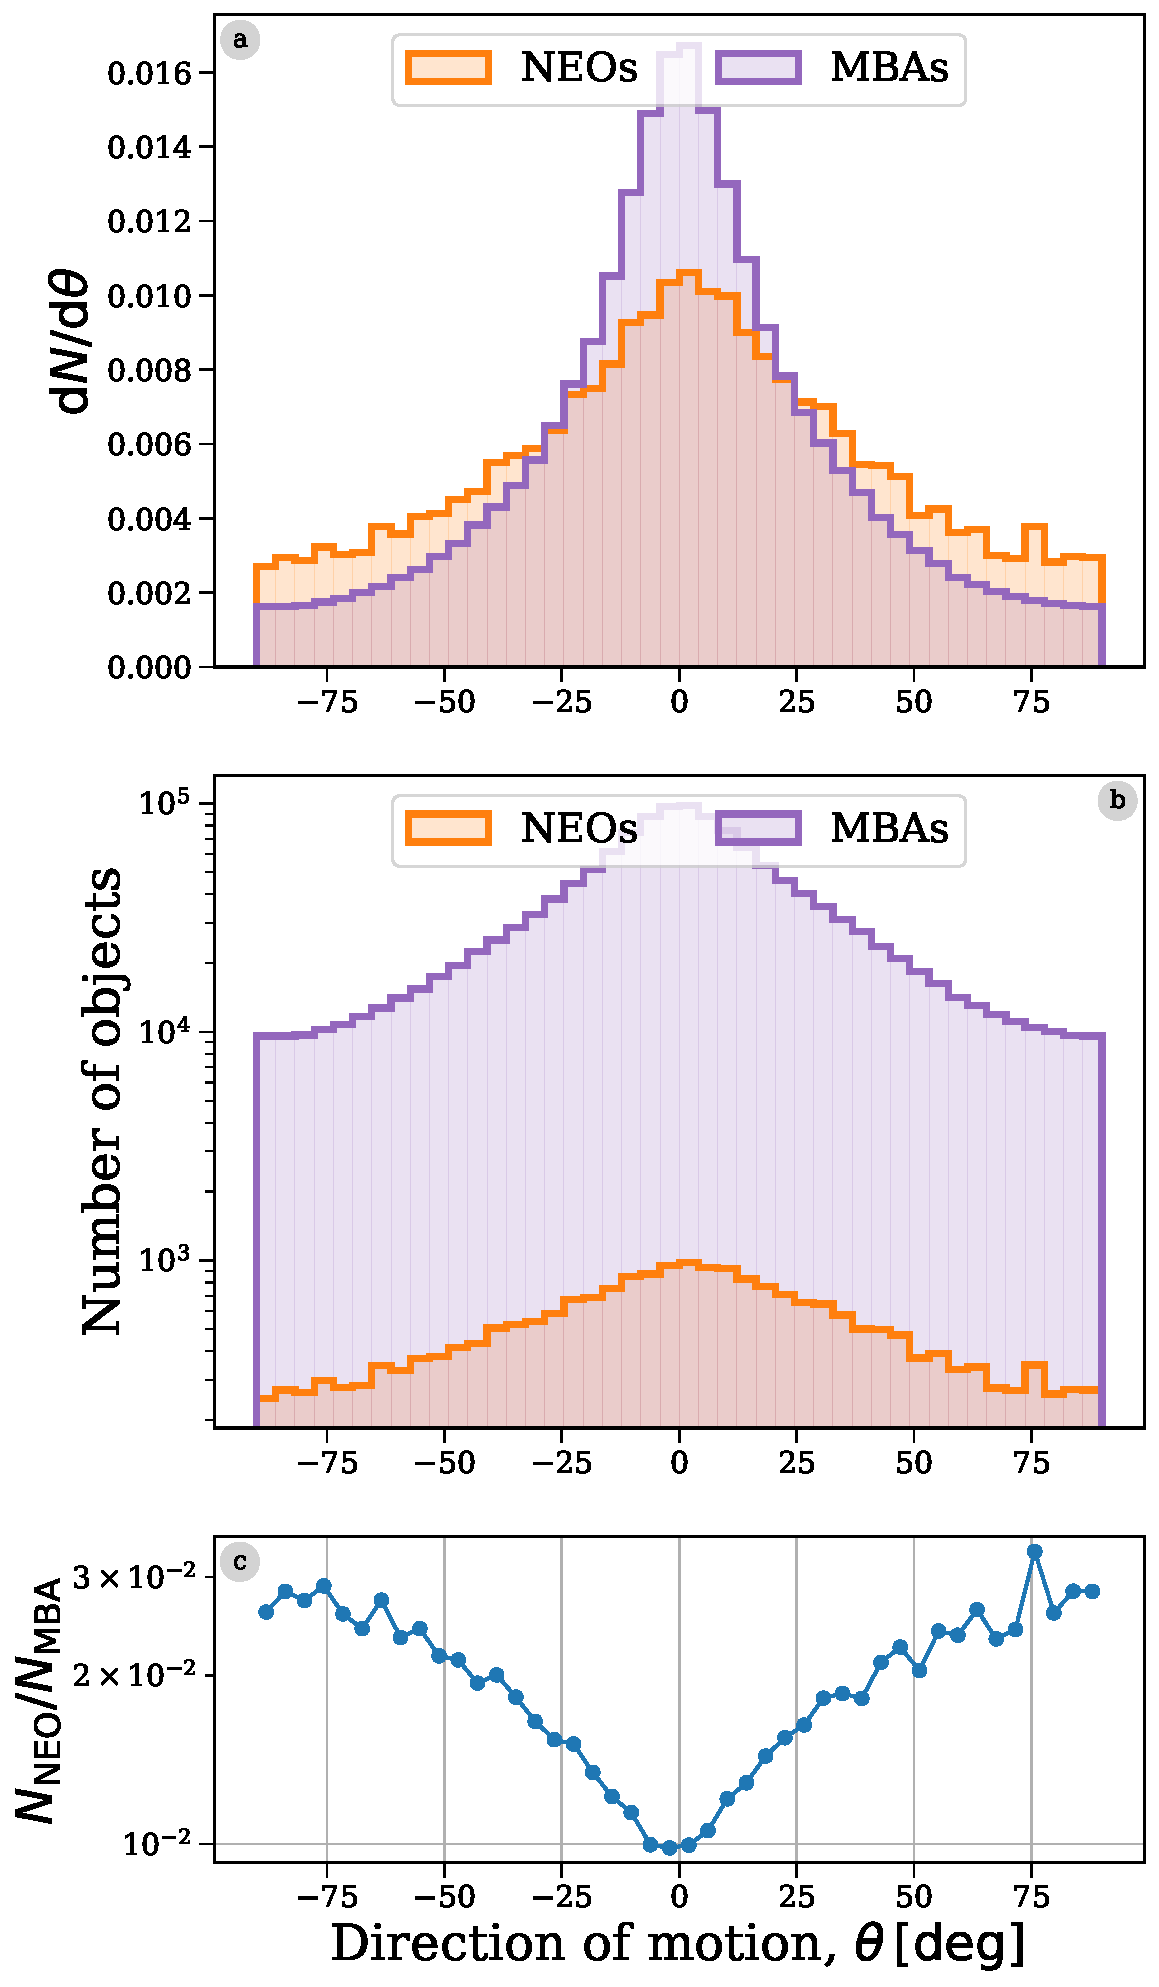
\includegraphics[width=\columnwidth]{figures/direction_dist_highscore.pdf}
    \caption{As Figure~\ref{fig:digest2_should_be_scared}, but for direction of motion relative to the ecliptic plane and only for observations with a \dig{} score of at least 65.}
    \label{fig:dir_highscore}
\end{figure}

Given that MBAs are constrained to the ecliptic plane and are further away than NEOs, one would predict that their motion is generally along the ecliptic plane, whilst NEOs could move in any direction. We investigate this in Figure~\ref{fig:dir_highscore} with the direction of $\theta$, the angle of the motion vector relative to the ecliptic plane. The separation in distributions is less clear cut than with the ecliptic latitude but we still find that objects moving away from the ecliptic plane have a larger fraction of NEOs than those moving along the plane.

\begin{figure}[htb]
    \centering
    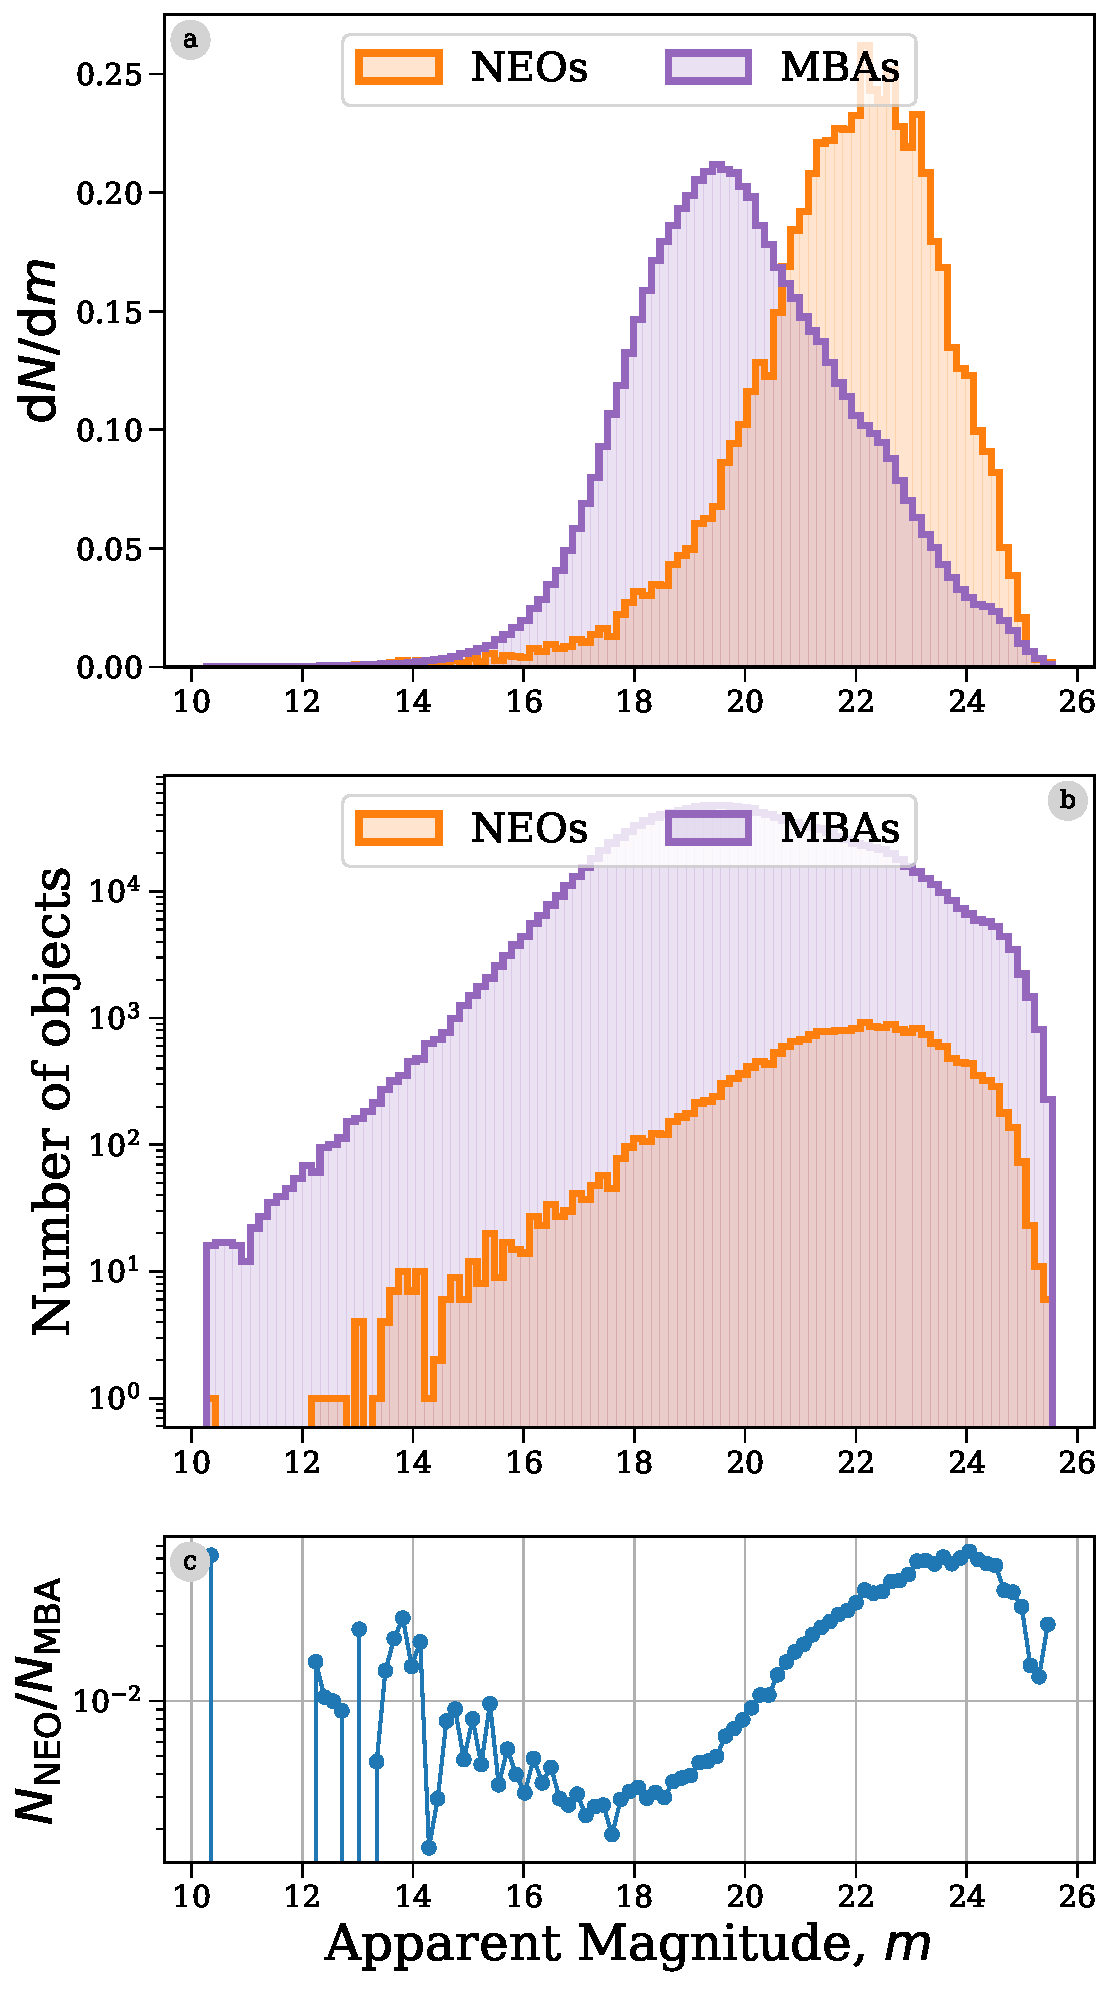
\includegraphics[width=\columnwidth]{figures/apparent_mag_dist_highscore.pdf}
    \caption{As Figure~\ref{fig:digest2_should_be_scared}, but for apparent V-band magnitude and only for observations with a \dig{} score of at least 65.}
    \label{fig:app_mag_highscore}
\end{figure}

\todo{apparent mag bit}

\section{Results}

\begin{itemize}
    \item Combine all 3 into 1 score, plot that up, compare to earlier one
    \item Decide on threshold and analyse performance with contingency matrix
    \item (Consider whether we could weight the different parameters differently to improve matters)
\end{itemize}

\section{Discussion}

\begin{itemize}
    \item Recommend sorting rather than just a threshold
    \item Coordination between groups will be important NEOFixer
\end{itemize}

\section{Conclusion}

\begin{itemize}
    \item Point out whether we did better :shrug:
\end{itemize}

\bibliographystyle{aasjournal}
\bibliography{refs}{}

\clearpage

\appendix

\section{Distributions of parameters for all observations}

The following plots show the distribution for the three parameters that we consider for the entire population of observations - in contrast to the earlier plots that only consider observations with a \dig{} score of at least 65. In general one can see that the distributions are less clear cut, in particular for the apparent magnitude distribution.

\begin{figure}[htb]
    \centering
    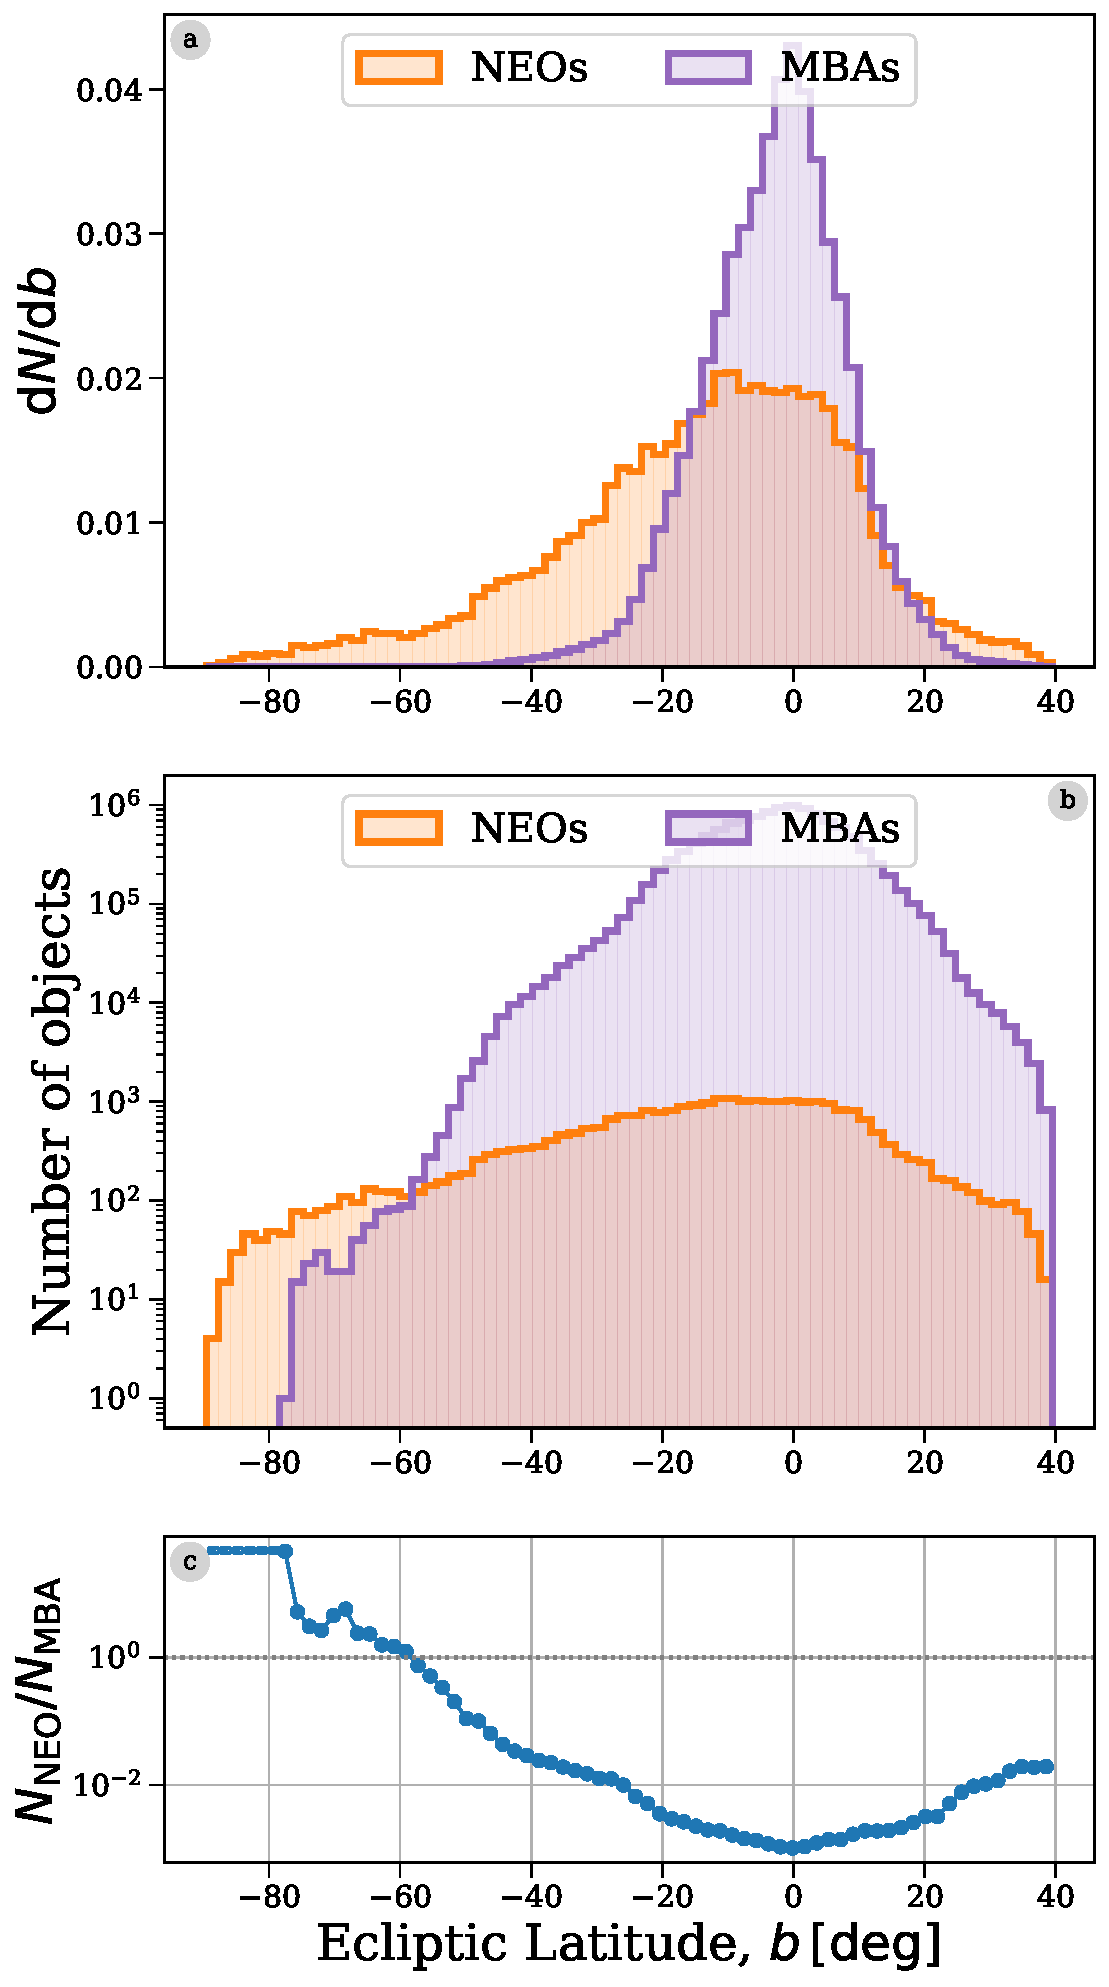
\includegraphics[width=\columnwidth]{figures/ecliptic_latitude_dist_all.pdf}
    \caption{As Figure~\ref{fig:digest2_should_be_scared}, but for ecliptic latitude.}
    \label{fig:ecl_lat_all}
\end{figure}

\begin{figure}[htb]
    \centering
    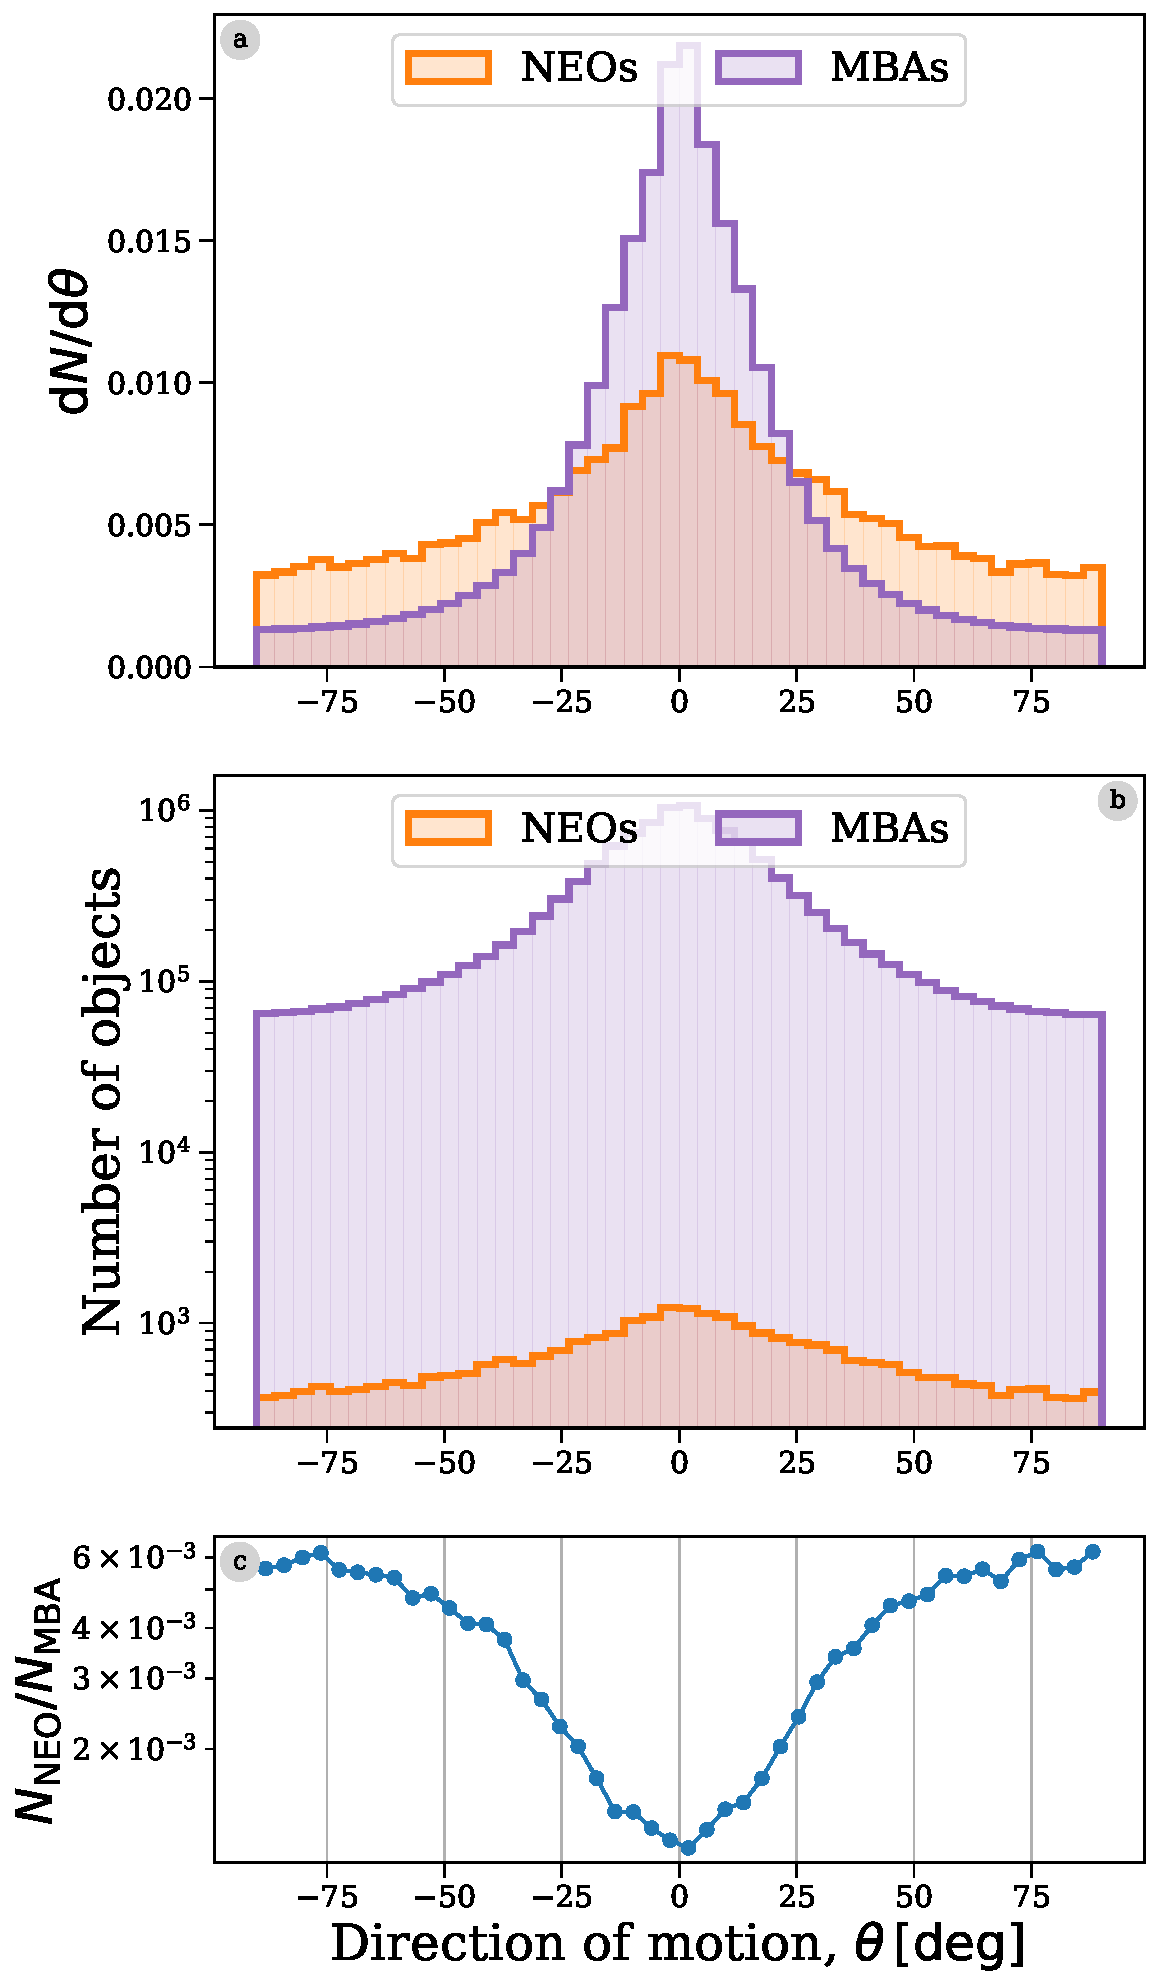
\includegraphics[width=\columnwidth]{figures/direction_dist_all.pdf}
    \caption{As Figure~\ref{fig:digest2_should_be_scared}, but for direction of motion relative to the ecliptic plane.}
    \label{fig:dir_all}
\end{figure}

\begin{figure}[htb]
    \centering
    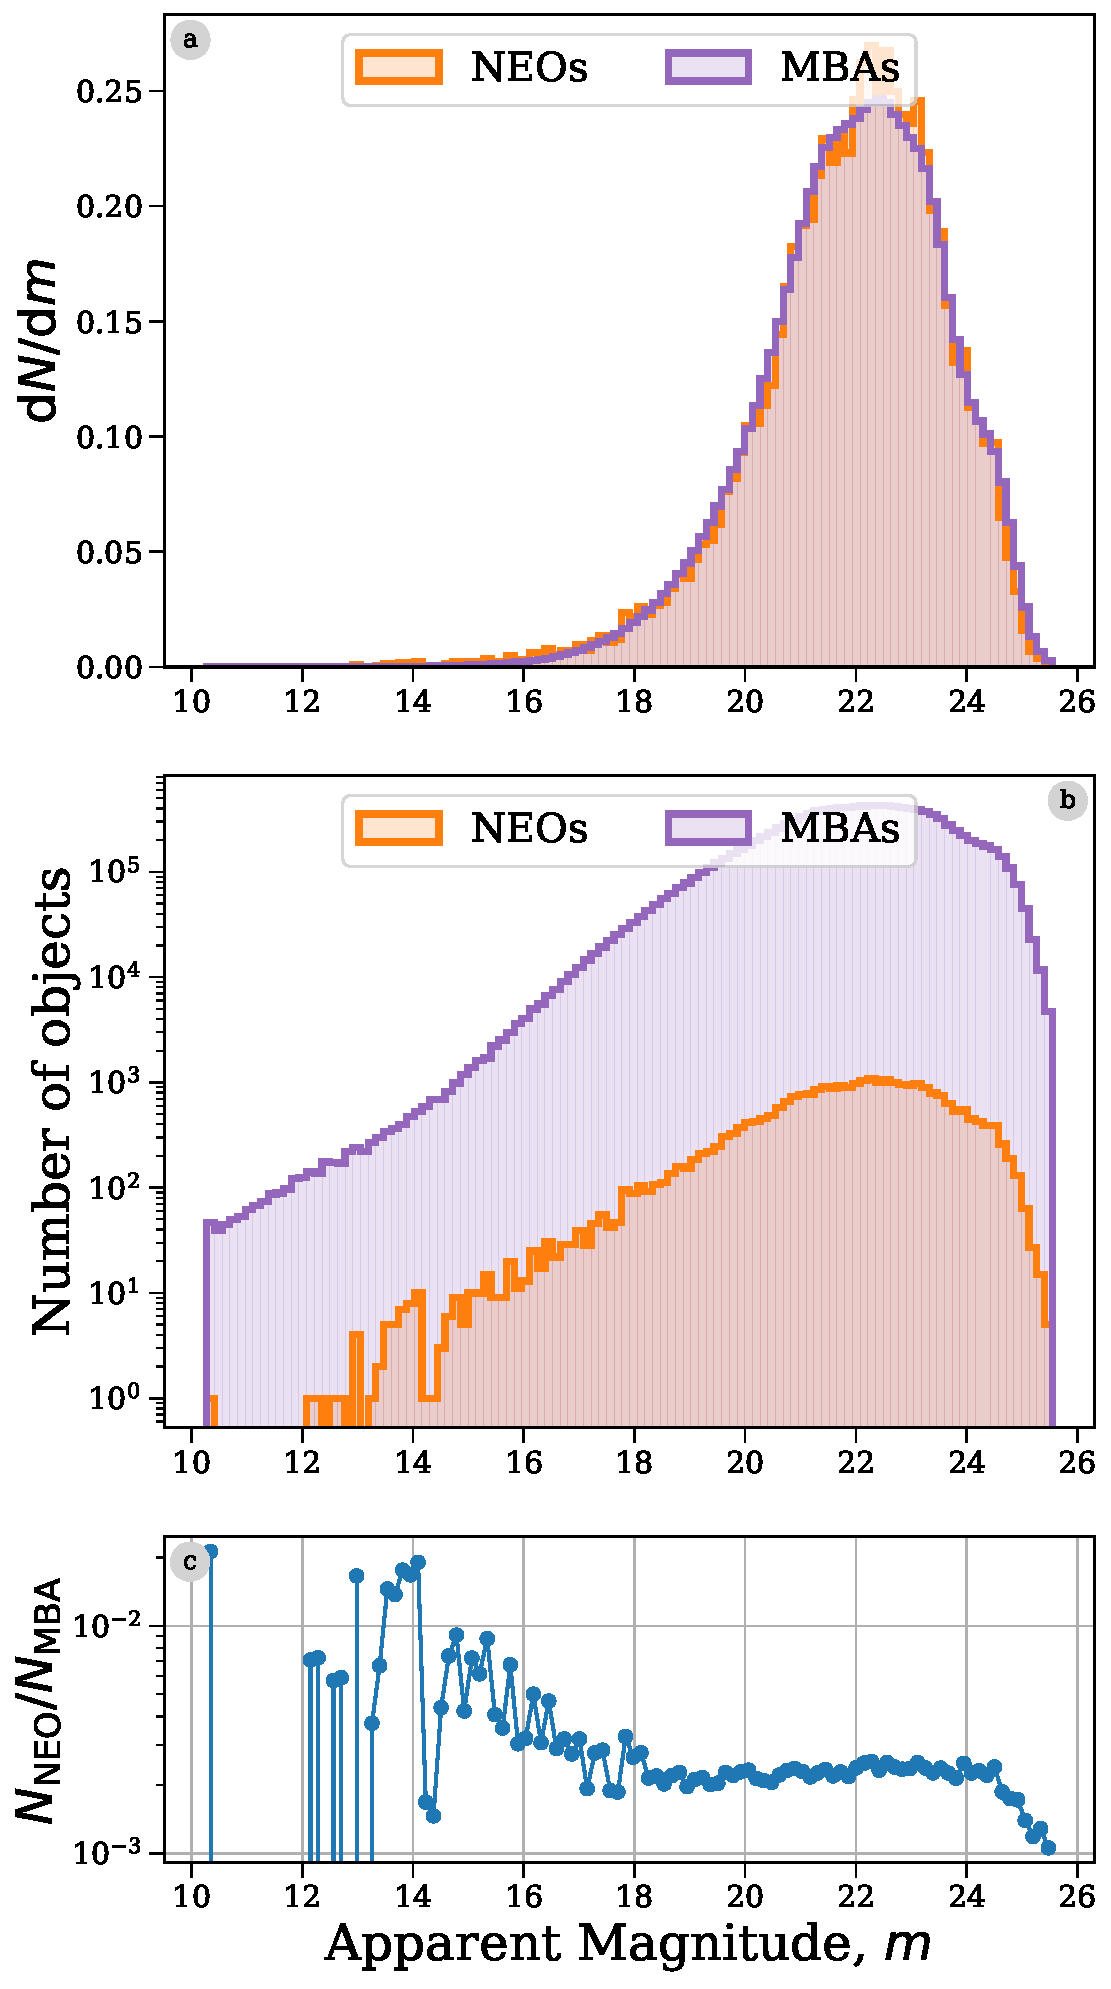
\includegraphics[width=\columnwidth]{figures/apparent_mag_dist_all.pdf}
    \caption{As Figure~\ref{fig:digest2_should_be_scared}, but for apparent V-band magnitude.}
    \label{fig:app_mag_all}
\end{figure}


\end{document}